\appendix
\chapter{Anexos}

\section{Anexo I: Mockups}

\begin{center}
  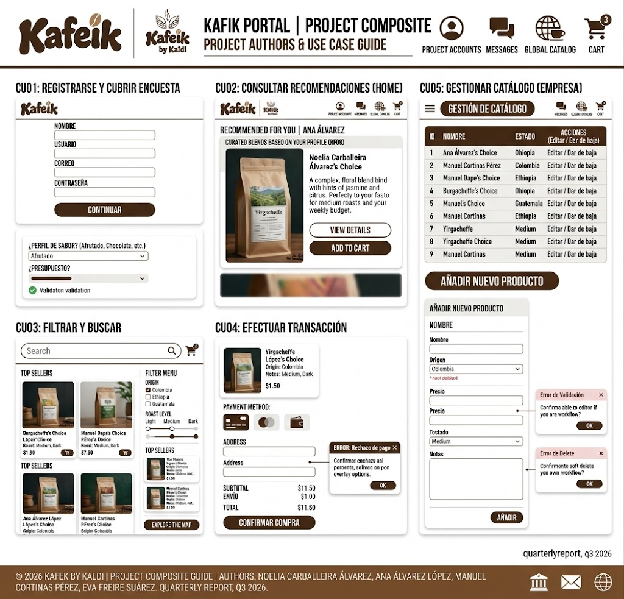
\includegraphics[width=\textwidth,keepaspectratio]{mockup-1.png}

  \textit{Mockup del portal de Kafeik y de sus principales pantallas}
\end{center}

\begin{center}
  
\includegraphics[width=\textwidth,keepaspectratio]{mockup-2.png}

  \textit{Mockup de los flujos de registro, recomendación, compra y gestión de catálogo}
\end{center}

\section{Anexo II: Uso de la IA}

Tal y como fue recomendado por el docente de la asignatura, se ha utilizado Inteligencia Artificial generativa para asistir tanto en la elaboración como en la corrección de este proyecto. En este anexo se explica cómo se han usado estas herramientas y en qué elementos están presentes.

\textbf{Logos:} el logo de Kafeik (el elefante) es producto de digitalizar con Gemini un dibujo hecho en papel. Se hizo así porque crear un dibujo digital a partir de uno en papel requeriría un número de horas excesivo para un elemento decorativo no determinante en el contenido.

\textbf{Mockups:} los mockups de la aplicación, logos y productos fueron generados con Gemini basándose en especificaciones sobre la estética visualizada para la empresa, la interfaz y otros factores.

\textbf{Detección de incoherencias:} se utilizó ChatGPT y Gemini para verificar y consolidar la coherencia y cohesión del documento mediante prompts como ``Señala todos los errores que encuentres en base a este criterio de corrección'', ``Señala las incoherencias entre apartados del siguiente documento'' o ``Critica la estructura y forma del documento''. Esto permitió detectar pequeñas incoherencias y estructurar el documento de forma más comprensible.

\textbf{Refinación de diagramas:} los diagramas de secuencia fueron inicialmente generados con Claude en PlantUML a partir de los workflows de los casos de uso 2--5. Un miembro del equipo eliminó las incoherencias y los refinó, enviándolos de nuevo a Claude para una última verificación. El diagrama de casos de uso fue inicialmente generado en PlantUML con los actores y el resto fue realizado íntegramente por un miembro del equipo.
